\documentclass[12pt, letterpaper]{article}
\usepackage{setspace}
\usepackage{amsfonts}
\usepackage{amsmath}
\usepackage{amsthm}
\usepackage{cancel}
\usepackage{thmtools}
\usepackage{multicol}
\usepackage[utf8]{inputenc}
\usepackage{graphicx}
\usepackage{titlesec}
\usepackage{float}
\usepackage[margin=1in]{geometry}
\usepackage[shortlabels]{enumitem}
\usepackage{gensymb}
\allowdisplaybreaks
\declaretheoremstyle[
	spaceabove=\topsep, spacebelow=\topsep,
	headfont=\normalfont\bfseries,
	notefont=\bfseries, notebraces={}{},
	bodyfont=\normalfont\itshape,
	postheadspace=0.5em,
	name={\ignorespaces},
	numbered=no,
	headpunct=:]{mystyle}
\newcommand{\Mod}[1]{\ (\mathrm{mod}\ #1)}
\declaretheorem[style=mystyle]{theorem}
\title{Automated Classification of Text-Based Math Questions Using LSTM Networks}
\author{Joseph Newcomer}
\date{June-July, 2024}
\begin{document}
\maketitle
\tableofcontents\newpage
\section{Introduction}
The proliferation of online platforms dedicated to academic discussions has revolutionized the way students, educators, and researchers engage with and disseminate knowledge. Among these platforms, Math Stack Exchange stands out as a premier forum for mathematical discourse, offering a vast repository of questions and answers that span the full spectrum of mathematical fields. However, the sheer volume and diversity of content present a significant challenge in terms of organization and navigation. Efficiently categorizing questions according to their respective fields of mathematics can greatly enhance user experience, improve searchability, and facilitate targeted knowledge retrieval. This task in its current form is performed by the users, resulting in potential inconsistencies. Therefore, developing an automated system for the classification of mathematical questions could be helpful for a platform such as this.
\par The primary motivation behind this project is to leverage deep learning and particularly recurrent networks to address this challenge. By automating the classification process, I aim to streamline the organization of content on Math Stack Exchange, thereby making it easier for users to find relevant information. Additionally, an automated system can ensure greater consistency in classification, reducing the ambiguity and overlap that often arises when humans categorize content. This automated classification not only aids users but also provides insights into the distribution and trends of mathematical inquiries over time.
\par From a machine learning perspective, the task at hand is a multilabel classification problem. Unlike traditional classification tasks where each instance is assigned a single label, multilabel classification involves associating each instance with multiple labels. In the context of Math Stack Exchange, a single question can belong to multiple mathematical fields. For example, a question about a specific mathematical problem might simultaneously involve aspects of algebra, calculus, and differential equations. This multilabel nature adds complexity to the classification task, as the model must learn to recognize and predict the co-occurrence of multiple labels.
\par To tackle this problem, I employ Long Short-Term Memory (LSTM) networks, a type of recurrent neural network (RNN) well-suited for sequence prediction tasks. LSTMs are particularly effective in handling the inherent sequential nature of text data, allowing the model to capture dependencies and contextual information across words and sentences. By training an LSTM-based model on a dataset of Math Stack Exchange questions, I aim to build a robust classifier capable of accurately predicting the relevant mathematical fields for each question.






\section{Data}
\subsection{Data Gathering}
The initial and most crucial step of any machine learning process is to gather a comprehensive and representative dataset. The source of this data was Math Stack Exchange, a platform where users post questions and answers about various mathematical topics. To ensure the dataset's relevance and diversity, I targeted questions associated with the top 30 tags on the platform. The selection of these tags was based on their popularity and coverage across different fields of mathematics. Each tag represents a specific domain or topic within mathematics, such as calculus, linear algebra, or probability.
\par The data collection process involved web scraping, a technique used to extract large amounts of data from websites. For this project, I developed a custom scraper to navigate Math Stack Exchange and extract questions tagged with my selected top 30 tags. The goal was to gather approximately the top 10,000 questions for each tag, resulting in a total of around 235,000 questions\footnote{Note that this isn't 300,000 total questions since some of the questions will overlap}. This volume of data was chosen to strike a balance between the complexity and manageability of the classification task, ensuring that the problem remained sufficiently challenging while still feasible to train on a local machine with limited computational resources.
\par The scraping script was implemented using Python, leveraging libraries such as BeautifulSoup for parsing HTML content and requests for handling HTTP requests. Each question's title, body, and associated tags were extracted and stored in a structured format. This structured data would later facilitate efficient preprocessing and analysis.
\par Once the data was collected, an exploratory analysis was conducted to understand its characteristics and ensure its quality. The first aspect examined was the distribution of tags across the dataset. The tag distribution, depicted in Figure 1, reveals that real-analysis and calculus were the most frequent tags, each appearing over 25,000 times. This high frequency indicates a strong interest in these fields among the Math Stack Exchange community as well as a larger overlap with other fields of mathematics. Other tags like probability, linear algebra, and integration also showed substantial representation, each with over 15,000 instances.
\begin{figure}[H]
\centering
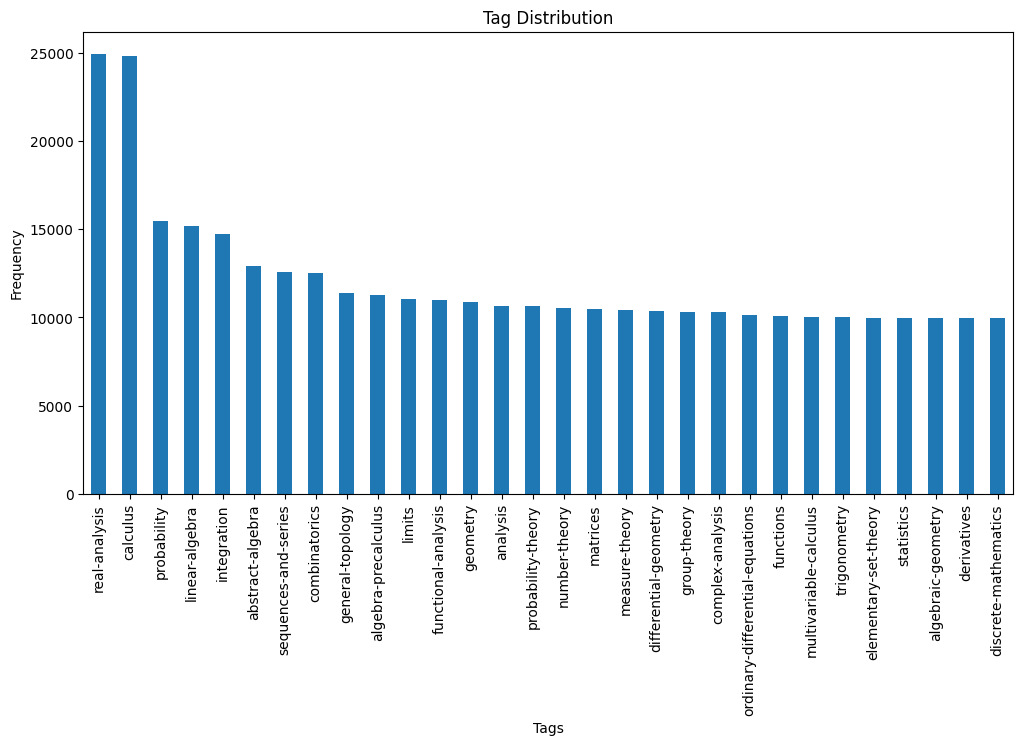
\includegraphics[scale=0.45]{../figs/exploratory_analysis/tag_distribution}
\caption{Distribution of tags across the Math Stack Exchange dataset}
\end{figure}
\par In addition to tag distribution, the length of question bodies was analyzed to understand the verbosity and complexity of the questions associated with each tag. Figure 2 presents the average lengths of question bodies for the top 30 tags. This analysis uncovered somewhat significant variations in question lengths, with tags like functional-analysis and complex-analysis having the longest average question bodies, indicating potentially more detailed and intricate queries. Figure 3 shows the distribution of lengths over all tags. 
\begin{figure}[H]
\centering
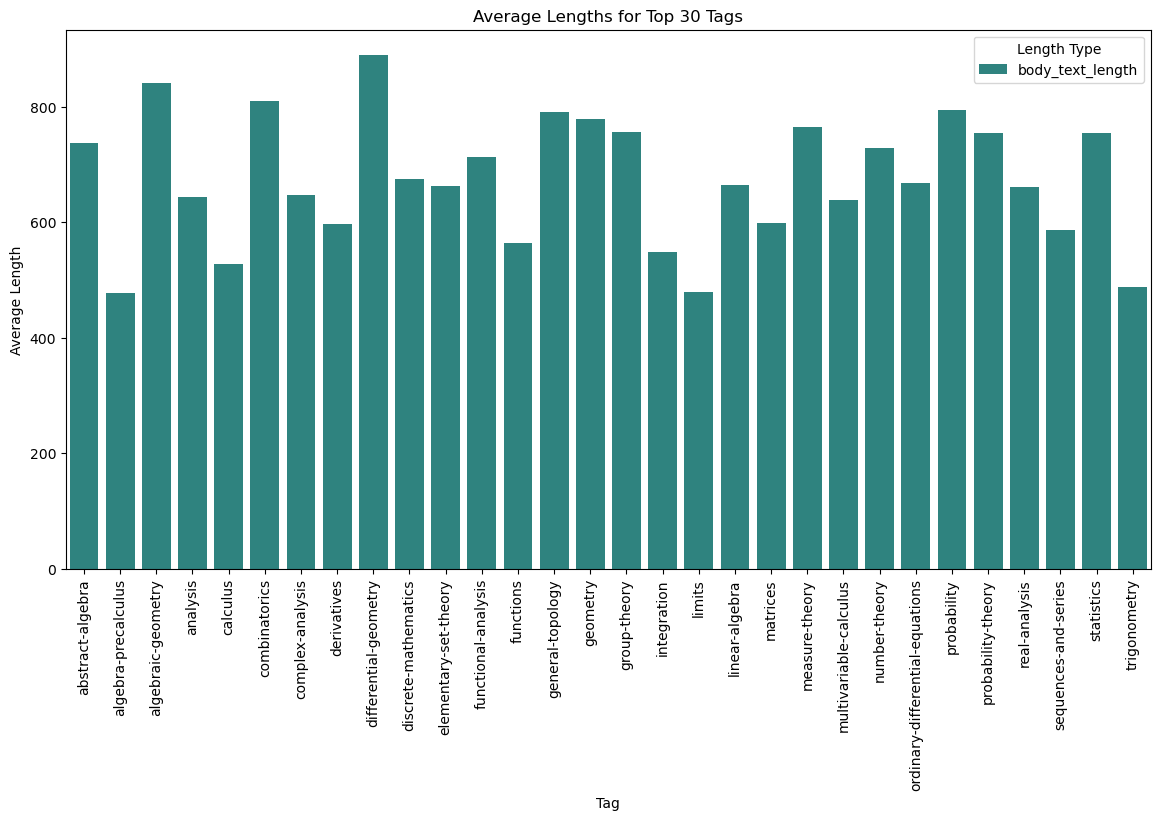
\includegraphics[scale=0.4]{../figs/exploratory_analysis/length_by_tag}
\caption{Distribution of question lengths across tags}
\end{figure}
\begin{figure}[H]
\centering
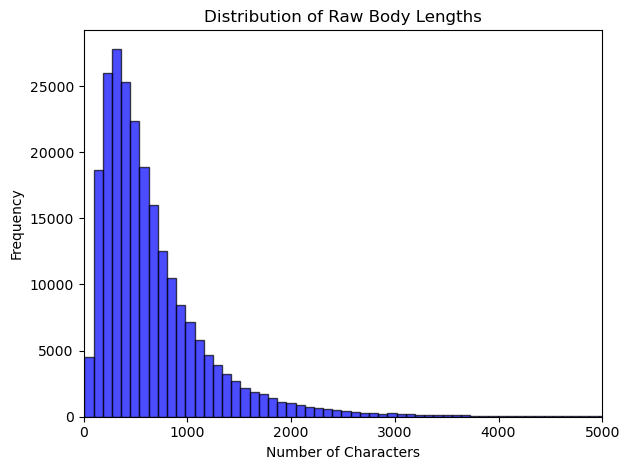
\includegraphics[scale=0.6]{../figs/exploratory_analysis/length_distribution}
\caption{Overall distribution of question lengths}
\end{figure}
\par A word cloud was also generated to visualize the most common words appearing in the bodies of the questions. Figure 4 highlights that terms related to proof-based mathematical questions such as "prove," "show," and "find," were predominant. This is unsurprising given the mathematical nature of the platform. However, this is important since, generally speaking, these words take on a different context in day-to-day speech. This is true of many of the other words represented in the word cloud, such as "set", "function", "group", etc. This will be important when it comes time to choose an embedding for these words for use in the LSTM network.
\begin{figure}[H]
\centering
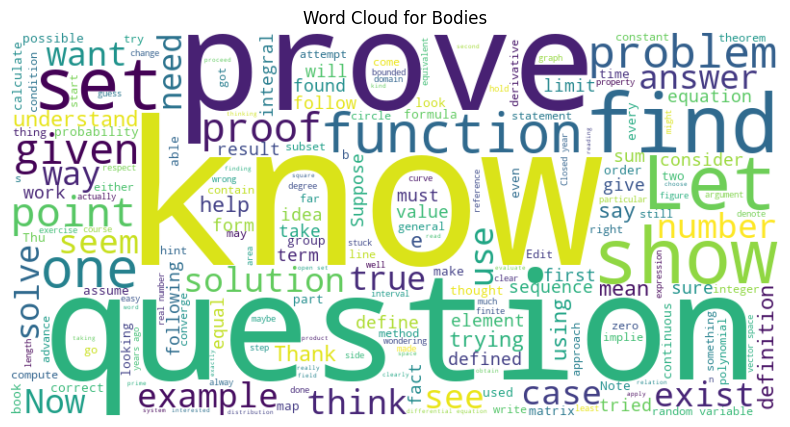
\includegraphics[scale=0.6]{../figs/exploratory_analysis/body_wordcloud}
\caption{Word Cloud of body text}
\end{figure}
\par The final component of the data gathering analysis involved examining the correlations between tags. The tag correlation matrix, shown in the fourth figure, provides insights into the co-occurrence patterns of tags within questions. This matrix reveals how often pairs of tags appear together in the same question, indicating potential overlaps between different mathematical fields. For instance, high correlations were observed between tags such as linear-algebra and matrices, or calculus and integration, reflecting their inherent interconnections. Understanding these correlations is crucial for the multilabel classification task, as it helps in capturing the relationships between different labels. A question tagged with calculus is often related to topics covered under integration or differential equations, and a robust classifier must account for these correlations to accurately predict multiple relevant tags.
\begin{figure}[H]
\centering
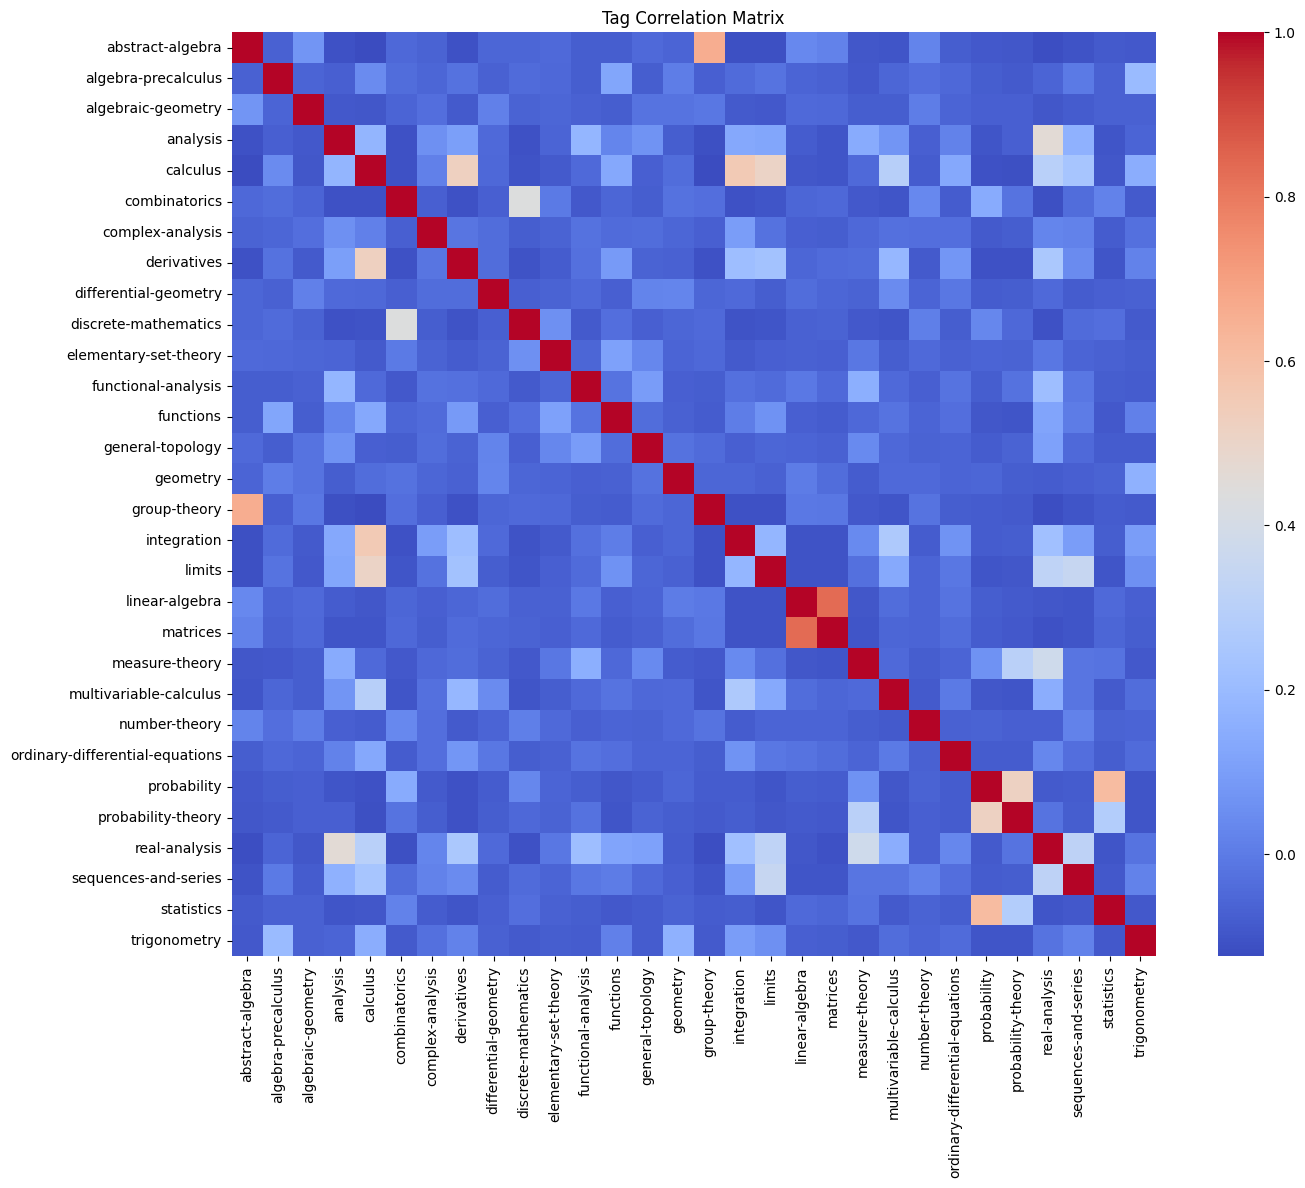
\includegraphics[scale=0.5]{../figs/exploratory_analysis/tag_corr_mat}
\caption{Tag correlation matrix}
\end{figure}
However, it is worth noting that the majority of these correlations are quite low. This suggests an inherent sparsity in the output labels of the dataset. Indeed, when checking the number of tags ascribed to each question in the dataset (shown in Figure 6), it can be seen that the vast majority of them are only 1 tag. This creates another challenge, as the sparsity of output labels will create an unbalanced dataset for training.
\begin{figure}[H]
\centering
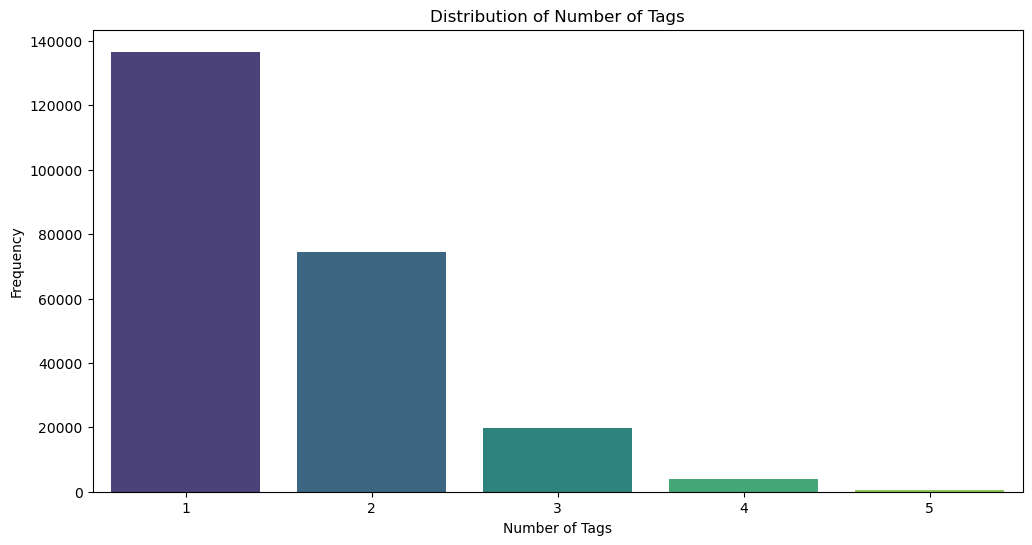
\includegraphics[scale=0.6]{../figs/exploratory_analysis/tag_number_distribution}
\caption{Distribution of number of tags}
\end{figure}
\subsection{Preprocessing}
The final step before model training was preprocessing. The primary goal of the preprocessing in this project was to standardize and clean the text, ensuring it was in a suitable format for the LSTM-based model. Given the nature of mathematical questions on Math Stack Exchange, a significant portion of the text included LaTeX expressions which needed to be handled appropriately. Directly processing LaTeX code can introduce noise and complexity into the text data. Therefore, the first step in preprocessing was to identify and replace all LaTeX expressions with a placeholder tag, <LATEX>. This approach preserves the structure and intent of the original question while simplifying the text data. 
\par The next step was tokenization, which involves splitting the text into individual words or tokens. This process was performed using the Natural Language Toolkit (NLTK) tokenizer package in Python. Tokenization facilitates the conversion of text into a sequence of tokens that can be processed by the LSTM model. Additionally, all tokens were converted to lowercase to ensure uniformity and to reduce the dimensionality of the text data. This normalization step helps in treating words like "Math" and "math" as the same token, thereby improving the consistency of the dataset.



\section{Model Design}
\subsection{LSTM Architecture}
The core of the classification system is a deep learning model based on the Long Short-Term Memory (LSTM) networks. LSTMs are a type of recurrent neural network (RNN) designed to handle sequential data and capture long-range dependencies, making them well-suited for text classification tasks. For this project, I implemented a two-layer LSTM architecture, chosen for its balance between complexity and performance. Each LSTM layer is followed by a dropout layer, which serves as a regularization technique to prevent overfitting by randomly setting a fraction of input units to zero during training.

The input layer of the model accepts a maximum sequence length of 500 words, which was determined to be a sufficient length to capture the essence of almost every question without introducing excessive computational overhead. The model's hyperparameters, including the learning rate, dropout rate, batch size, and the number of hidden units in the LSTM layers, were adjustable. This flexibility allowed me to fine-tune the model for optimal performance. The architecture leverages the sequential nature of LSTMs to effectively process the tokenized text data, ultimately producing a set of predictions corresponding to the various mathematical fields.
\subsection{Evaluation Metrics}
 Evaluating the performance of a multilabel classifier requires careful consideration of the metrics used. Given the complexity of the problem, subset accuracy, which measures the proportion of exact matches between predicted and true label sets, is highly challenging to optimize due to its stringent nature. Conversely, Hamming loss, which counts the fraction of incorrectly predicted labels, is overly lenient in sparse output scenarios, where the majority of possible labels are not present.
\par As a balanced alternative, I adopted the micro-averaged F1 score as my primary evaluation metric. The micro-averaged F1 score aggregates contributions from all classes to compute the overall precision and recall, providing a comprehensive measure of the model's performance across all tags. This metric is particularly suitable for this task, as it accounts for both false positives and false negatives in a balanced manner. Additionally, we placed a secondary focus on precision due to the higher impact of false positives in sparse output situations, where incorrect tags can significantly detract from the model's utility and reliability.
\subsection{Word Embeddings}
To transform the input text into a numerical format suitable for LSTM processing, word embeddings were employed. Word embeddings map words to continuous vector spaces, capturing semantic similarities between words. Two competing embeddings were evaluated on a smaller, single-layer LSTM model: a custom 300-dimensional Word2Vec embedding trained on our dataset, and Google's pre-trained Word2Vec model trained on the Google News corpus.
\par The custom Word2Vec model was trained specifically on the Math Stack Exchange data, ensuring that it captured the unique linguistic patterns and terminology prevalent in mathematical questions. In contrast, Google's pre-trained model provided a broader but less domain-specific representation. Performance comparisons indicated that the custom embedding slightly outperformed the pre-trained model on our primary evaluation metrics, including the micro-averaged F1 score and precision.\footnote{It is also worth noting that these embeddings served solely as initial conditions for the network. They were allowed to be trainable throughout the process in order to optimize for the task as best as possible.} This improvement, although modest, justified the use of the custom Word2Vec embedding for the final model, as it better aligned with the specific context and vocabulary of the dataset.
\section{Results and Conclusion}
\subsection{Final Model Results}
Along with F1-score and precision, the performance of my LSTM-based classifier was evaluated using Hamming loss, subset accuracy, and recall as well. After training the final model for 25 epochs, the final model achieved a micro-averaged F1 score of 0.64 and a precision of 0.73. These metrics indicate a robust performance given the complexity of the multilabel classification task at hand. These results, along with the metrics corresponding to the initial two models, are shown below:
\begin{figure}[H]
\centering
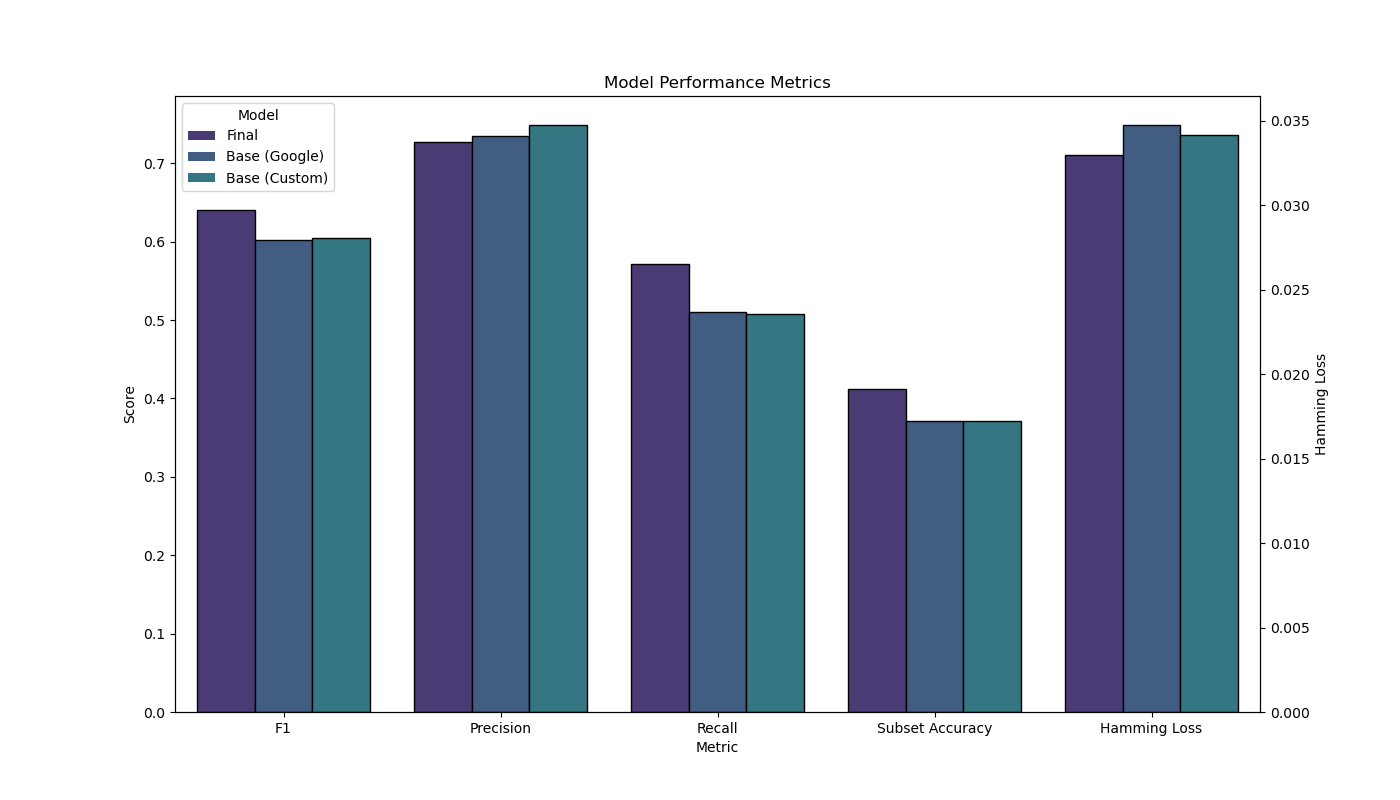
\includegraphics[scale=0.45]{../figs/recurrent_nn/final_performance}
\caption{Final model results as well as the results from the two base models trained on the custom and Google embedding matrices.}
\end{figure}
Achieving an F1 score of 0.64 signifies a balanced trade-off between precision and recall, indicating that the model is effectively identifying relevant tags without being overly conservative. The precision of 0.73 is particularly noteworthy, as it highlights the model's ability to minimize false positives. This is crucial in the context of sparse outputs, where assigning incorrect tags can significantly degrade the quality and utility of the classification system.
\par The comparison between the final model and the two base models—one using Google's pre-trained Word2Vec embeddings and the other using custom-trained embeddings—further underscores the efficacy of this approach. The final model, which incorporated the domain-specific custom embeddings, outperformed both base models across all metrics.

\subsection{Future Improvements}
While the final results are better than the initial models' results, there is still quite a bit of room for improvement. The limitations of my local computing power are the key issue in creating larger and more robust models. With more data and more LSTM layers, I believe it would be possible to push the F1-score to above 0.7 and the subset accuracy to over 50\%. However, with the current final iteration already taking over a day to train on my local machine, adding another layer or gathering more data is simply infeasible.
\par It is also possible that more advanced architectures could create more promising results. Bidirectional LSTMs or ensemble methods using other deep learning techniques could prove to be even more effective than a simple LSTM-based model. However, as previously stated, this would also require a lot more computing power or time, neither of which I have right now.
\par In summary, the results validate the effectiveness of my LSTM-based approach for classifying mathematical questions by field. The model's performance, particularly in terms of precision and the balanced F1 score, underscores its potential utility. However, there is quite a bit of room for improvement, and in a setting where computing power isn't a limiting factor, some dramatic improvements might be able to be made by expanding the model and scraping more data. 

















\end{document}